This section provides two case studies that showcase the effectiveness and applicability of our proposed approach. In these studies, we investigate the properties and performance of the approach using streamed benchmark system data and signals from IoT devices in a microgrid system.  The successful deployment demonstrates that this approach is suitable for existing process automation infrastructure.

The case studies were realized using Python 3.10.1 on a machine employing an 8-core Apple M1 CPU and 8 GB RAM.

\subsection{Benchmark}\label{AA:Benchmark}
In this subsection, we compare the proposed method with standard adaptive unsupervised detection methods. Two of the most well-known methods, providing iterative learning capabilities over multivariate time-series data are One-Class Support Vector Machine (OC-SVM) and Half Spaced Trees (HS-Trees). Both methods represent the state of the art for cases of anomaly detection on dynamic system data. Comparison is conducted on real benchmarking data, annotated with labels of whether the observation was anomalous or normal. The dataset of Skoltech Anomaly Benchmark (SKAB) \cite{skab2020} is used for this purpose. It represents a combination of experiments with the behavior of rotor imbalance as a subject to various functions introduced to control action as well as slow and sudden changes in the amount of water in the circuit. The system is described by 8 features. The data were preprocessed according to best practices for the given method, namely: standard scaling for OC-SVM, normalization for HS-Trees, and no scaling for the proposed method. The optimal quantile threshold value for both reference methods is found using grid search. Results are provided within Table \ref{tab:perf_comp}, evaluating F1 score, Recall and Precision. Value of 100\% at each metric represents a perfect detection. The latency represents the average computation time per sample of the pipeline including training and data preprocessing. 

\begin{table}[htbp]
  \caption{Metrics evaluation on SKAB dataset}
  \begin{center}
  \label{tab:perf_comp}
  \begin{tabular}{|c|c|c|c|c|}
    \hline
    Metric & RAID & OC-SVM & HS-Trees \\
    \hline
    F1 [$\%$] & $\boldsymbol{48.70}$ & 44.42 & 34.10 \\
    \hline
    Recall [$\%$] & 49.90 & $\boldsymbol{56.67}$ & 32.57 \\
    \hline
    Precision [$\%$] & $\boldsymbol{47.56}$ & 36.52 & 35.77 \\
    \hline
    Avg. Latency [ms] & 1.55 & 0.44 & $\boldsymbol{0.21}$ \\
    \hline
  \end{tabular}
  \end{center}
\end{table}

The results in Table \ref{tab:perf_comp}suggest that our algorithm provides slightly better performance than reference methods. Based on the Scoreboard for various algorithms on SKAB's Kaggle page, our iterative approach performs comparably to the evaluated batch-trained model. Such a model has all the training data available before prediction unlike ours, evaluating the metrics iteratively on a streamed dataset.

\subsection{Battery Energy Storage System (BESS)}\label{AA:BESS}
In the second case study, we verify our proposed method on BESS. The BESS reports measurements of State of Charge (SoC), supply/draw energy set-points, and inner temperature, at the top, middle, and bottom of BESS. Tight battery cell temperature control is needed to optimize performance and maximize the battery's lifespan. Identifying anomalous events and removal of corrupted data might yield significant improvement on the process control level. 

The default sampling rate of the signal measurement is 1 minute. However, network communication of the IoT devices is prone to packet dropout, which results in non-uniform sampling. The data are normalized to the range $[0, 1$] to protect the sensitive business value. The proposed approach is deployed to the existing infrastructure of the system, allowing real-time detection and diagnosis of the system.

\begin{figure}[htbp]
\centerline{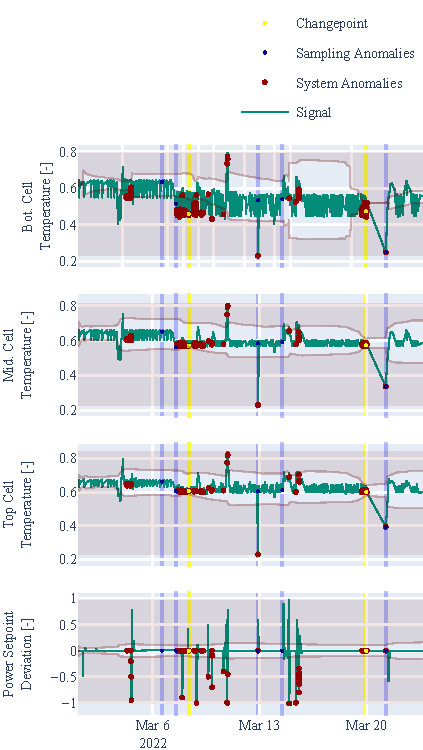
\includegraphics{figures/system_thresh.pdf}}
\caption{Time Series of BESS measurements (green line) of process variables. Non-uniform ticks on the x-axis mark days of interest (NOTE: some marks are hidden due to the readability). The y-axis renders the normalized process variables. System anomalies are marked as red dots. Non-uniform sampling is detected at blue vertical lines. Yellow vertical lines denote changepoint adaptation}
\label{fig:process}
\end{figure}

Fig. \ref{fig:process} depicts the operation of the BESS over March 2022. Multiple events of anomalous behavior were reported by the operators, that are observable through a sudden or significant shift in measurements in a given period. As the first step, the model was initialized, following Subsection \ref{init} system parameters were selected as $t_e = 4$ days and $T = -25$ for the expiration period and threshold accordingly. By design, the first 3 days are within the grace period, during which the model is calibrated.

The deployment and operation of the anomaly detection system were successful as shown by its adaptation of changepoint on 7\textsuperscript{th} March 2022 that appeared due to the relocation of the battery storage system outdoors. The model was adapted online based on Subsection \ref{train}. A dramatic shift in environmental conditions changed the dynamics of the system's temperature. However, new behavior was adopted by the top-level anomaly isolation system within two days, significantly reducing the number of alerts afterward. Interestingly, calibration of the system, as shown in deviations of setpoint from real power demand and multiple peaks in temperature were captured as well. 

The system identified 5 deviations in sampling, denoted by the blue line in Fig. \ref{fig:process}. The longest packet loss observed happened across 20\textsuperscript{th} March up to 21\textsuperscript{st}. Unexpectedly, the change point detection module identified start of the loss as a changepoint, followed by the detector of deviations in sampling that could only capture the event with the next observation after the loss. Red dots represent anomalies at the system level given by equation \eqref{eq:anomaly}. The dynamic signal limits are surpassed in one or multiple signals during the system's anomalies. Moreover, shifts in the relationship between variables are considered by the model based on the correlation matrix.
